\documentclass[11pt,aspectratio=169]{beamer}

\usepackage{amsmath,amssymb,bm}
\usepackage{booktabs}
\usepackage{tikz}
\usetikzlibrary{arrows.meta,positioning,calc}

\usetheme{default}
\setbeamertemplate{navigation symbols}{}
\setbeamertemplate{headline}{}
\setbeamertemplate{footline}{%
  \leavevmode
  \hbox{%
    \begin{beamercolorbox}[wd=\paperwidth,ht=2.6ex,dp=1.1ex,right]{page number in head/foot}%
      \insertframenumber/\inserttotalframenumber\hspace{0.35cm}
    \end{beamercolorbox}%
  }%
}
\setbeamertemplate{frametitle}{\vspace{0.25cm}\insertframetitle\par\vspace{0.08cm}\hrule}
\setbeamercolor{normal text}{fg=black,bg=white}
\setbeamercolor{frametitle}{fg=black,bg=white}
\setbeamercolor{structure}{fg=black}
\setbeamersize{text margin left=0.7cm,text margin right=0.7cm}

\newcommand{\dd}{\,\mathrm{d}}
\newcommand{\Om}{\Omega}
\newcommand{\GamD}{\Gamma_D}
\newcommand{\GamN}{\Gamma_N}
\newcommand{\Th}{\mathcal T_h}
\newcommand{\Fh}{\mathcal F_h}
\newcommand{\Vzero}{\mathcal V_0}
\newcommand{\Vhzero}{\mathcal V_{h,0}}
\newcommand{\Qh}{\mathcal Q_h}
\newcommand{\norm}[2][]{\left\lVert#2\right\rVert_{#1}}
\newcommand{\seminorm}[2][]{\left\lvert#2\right\rvert_{#1}}
\newcommand{\grad}{\nabla}
\newcommand{\divg}{\nabla\!\cdot}
\newcommand{\bn}{\bm n}
\newcommand{\bq}{\bm q}

\begin{document}

\begin{frame}[plain]
  \centering\vfill
  {\LARGE\bfseries Residual Estimator and Reliability\par}
  \vspace{0.45cm}
  {\large Element and facet residuals, local indicators, and an energy-error
  bound\par}
  \vfill
\end{frame}

\begin{frame}{Lecture outline}
We begin with the elementwise integration-by-parts formula obtained in the
previous lecture.

\begin{enumerate}
  \item Regroup element-boundary terms into interior, Neumann, and Dirichlet
  facet contributions.
  \item Compute element and facet residuals in one and two dimensions.
  \item Derive the mesh-size weights in the residual estimator.
  \item Prove that the estimator gives a reliable upper bound for the energy
  error.
\end{enumerate}

The two worked examples show where the element and facet terms enter. The
reliability proof then explains why these computable terms control the unknown
error.
\end{frame}

\begin{frame}{Review: residual and Galerkin orthogonality}
For the diffusion problem,
\[
  R(u_h;v)=\ell(v)-a(u_h,v),
  \qquad v\in\Vzero.
\]
If $e=u-u_h$, then the continuous equation gives
\[
  R(u_h;v)=a(e,v),
  \qquad
  \norm[a]{e}^2=R(u_h;e).
\]
The finite element equation gives
\[
  R(u_h;v_h)=0
  \qquad\forall v_h\in\Vhzero.
\]
Thus the residual measures the part of the continuous problem not tested by
the discrete space. Galerkin orthogonality will later allow us to replace an
unknown test function by its finite element approximation error.
\end{frame}

\begin{frame}{Review: integration by parts on each element}
The previous lecture stopped after applying Green's formula separately on
every element:
\[
\begin{aligned}
 \int_{\mathcal K_e}k\grad u_h\cdot\grad v\,\dd x
 ={}&-\int_{\mathcal K_e}\divg(k\grad u_h)v\,\dd x\\
 &+\int_{\partial\mathcal K_e}
 (k\grad u_h\cdot\bn_e)v\,\dd s.
\end{aligned}
\]
The first term measures the balance defect inside $\mathcal K_e$. The second
term lies on the element boundary.

\vspace{0.2cm}
The next step is to sum over all elements and determine what the boundary
terms become on each class of facet.
\end{frame}

\begin{frame}{After summing, every element boundary must be classified}
Substituting the elementwise identity into the residual gives
\[
\begin{aligned}
R(u_h;v)={}&
\sum_e\int_{\mathcal K_e}
\bigl(f+\divg(k\grad u_h)\bigr)v\,\dd x\\
&-\sum_e\int_{\partial\mathcal K_e}
(k\grad u_h\cdot\bn_e)v\,\dd s
+\int_{\GamN}qv\,\dd s.
\end{aligned}
\]

The first line is already separated by element. In the second line:
\begin{itemize}
  \item an interior facet appears twice, once from each neighboring element;
  \item a Neumann facet appears once and combines with the prescribed-flux
  integral; and
  \item a Dirichlet facet contributes zero because $v=0$ on $\GamD$.
\end{itemize}
\end{frame}

\begin{frame}{Interior facet: the two outward normals have opposite signs}
Let $\mathcal F=\partial\mathcal K^+\cap\partial\mathcal K^-$. The outward
normals are $\bn_{\mathcal F}$ for $\mathcal K^+$ and
$-\bn_{\mathcal F}$ for $\mathcal K^-$. The two boundary terms are
\[
\begin{aligned}
&-\int_{\mathcal F}
  k\grad u_h^+\cdot\bn_{\mathcal F}\,v\,\dd s
-\int_{\mathcal F}
  k\grad u_h^-\cdot(-\bn_{\mathcal F})\,v\,\dd s\\
&\qquad=-\int_{\mathcal F}
  \bigl(k\grad u_h^+-k\grad u_h^-\bigr)
  \cdot\bn_{\mathcal F}\,v\,\dd s.
\end{aligned}
\]
Because $v\in H^1(\Om)$ has the same boundary value on the shared facet when
approached from either conforming element, the same $v$ appears in both terms.
The coefficient of $v$ in the resulting facet integral is the negative
normal-flux jump. Define the interior-facet residual by
\[
  j_{\mathcal F}
  =-[\![k\grad u_h\cdot\bn_{\mathcal F}]\!]_{\mathcal F}.
\]
\end{frame}

\begin{frame}{Boundary facets and the complete residual representation}
Define the computed vector flux element by element:
\[
  \bq_h=k\grad u_h.
\]
On a Neumann facet, the element-boundary term and prescribed-flux term give
\[
  j_{\mathcal F}
  =q-k\grad u_h\cdot\bn
  =q-\bq_h\cdot\bn.
\]
On a Dirichlet facet, $v=0$. Define
\[
  r_e=f+\divg(k\grad u_h)=f+\divg\bq_h.
\]
The residual is therefore
\[
\boxed{
R(u_h;v)=
\sum_e\int_{\mathcal K_e}r_ev\,\dd x
+\sum_{\mathcal F\in\Fh^{\mathrm{int}}\cup\Fh^N}
\int_{\mathcal F}j_{\mathcal F}v\,\dd s.}
\]
This is an exact identity, not an estimate.
\end{frame}

\begin{frame}{What the two residuals measure}
\begin{center}
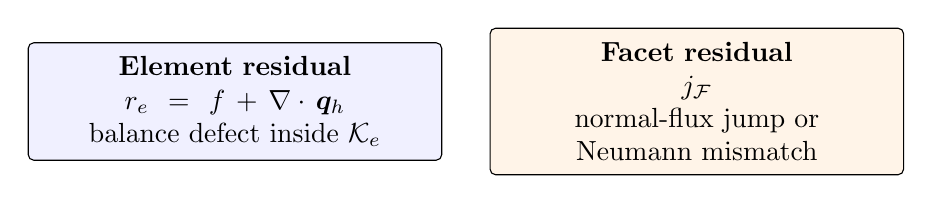
\begin{tikzpicture}[
  box/.style={draw,rounded corners=2pt,align=center,text width=4.9cm,
    minimum height=1.35cm,inner sep=5pt}]
  \node[box,fill=blue!6] (element) {\textbf{Element residual}\\
    $r_e=f+\divg\bq_h$\\
    balance defect inside $\mathcal K_e$};
  \node[box,fill=orange!9,right=0.6cm of element] (facet) {\textbf{Facet residual}\\
    $j_{\mathcal F}$\\
    normal-flux jump or Neumann mismatch};
\end{tikzpicture}
\end{center}

For $P_1$ elements and elementwise-constant $k$, $\grad u_h$ and
$k\grad u_h$ are constant on each element. Hence
\[
  \divg(k\grad u_h)=0,
  \qquad r_e=f|_{\mathcal K_e}.
\]
The element residual then reduces to the prescribed source. The
computed-gradient information is contained in the facet residuals.
\end{frame}

\begin{frame}{Nonuniform 1D example: compute the residuals}
\[
  -u''=1\ \text{in }(0,1),
  \qquad u(0)=0,
  \qquad u'(1)=0,
  \qquad
  (U_1,U_2,U_3)=\left(0,\frac5{18},\frac12\right).
\]
\begin{center}
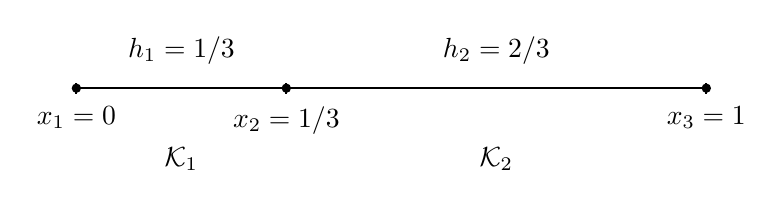
\begin{tikzpicture}[x=8.0cm,y=1cm]
  \draw[thick] (0,0)--(1,0);
  \foreach \x in {0,0.3333,1}{
    \draw[thick] (\x,-0.07)--(\x,0.07);
    \fill (\x,0) circle (1.7pt);
  }
  \node[below=3pt] at (0,0) {$x_1=0$};
  \node[below=3pt] at (0.3333,0) {$x_2=1/3$};
  \node[below=3pt] at (1,0) {$x_3=1$};
  \node[below=18pt] at (0.1667,0) {$\mathcal K_1$};
  \node[below=18pt] at (0.6667,0) {$\mathcal K_2$};
  \node[above=5pt] at (0.1667,0) {$h_1=1/3$};
  \node[above=5pt] at (0.6667,0) {$h_2=2/3$};
\end{tikzpicture}
\end{center}
\[
  u_h'|_{\mathcal K_1}=\frac56,
  \qquad
  u_h'|_{\mathcal K_2}=\frac13,
  \qquad r_1=r_2=1.
\]
In one dimension the facets are nodes. Thus
$j_2=1/3-5/6=-1/2$ and $j_3=0-1/3=-1/3$.
\end{frame}

\begin{frame}{What the 1D example shows}
For every test function $v$ with $v(0)=0$,
\[
  R(u_h;v)
  =\int_{\mathcal K_1}v\,\dd x
   +\int_{\mathcal K_2}v\,\dd x
   -\frac12v(x_2)-\frac13v(x_3).
\]
The residual therefore contains both the element terms and the two facet
terms.

\begin{columns}[T,onlytextwidth]
\begin{column}{0.49\textwidth}
\textbf{Effect of element size.}
\[
 h_e^2\norm[L^2(\mathcal K_e)]{r_e}^2=h_e^3,
 \qquad
 \norm[a,\mathcal K_e]{u-u_h}^2=\frac{h_e^3}{12}.
\]
Because $h_2=2h_1$, $\mathcal K_2$ contributes eight times as much to both
squared quantities.
\end{column}
\begin{column}{0.48\textwidth}
\textbf{Special feature of 1D.}
For $w=e-\mathcal I_h e$,
\[
  w(x_i)=0
\]
at every node. Thus the point-facet terms vanish from the 1D reliability
proof even though $j_2$ and $j_3$ are nonzero. For $d\geq2$, the facet terms
remain in the estimator.
\end{column}
\end{columns}
\end{frame}

\section{Residual estimator}

\begin{frame}[plain]
  \centering\vfill
  {\LARGE\bfseries Constructing a residual estimator\par}
  \vspace{0.4cm}
  {\large Remove the unknown error from the residual identity, identify the
  mesh-size weights, and obtain a computable upper bound.\par}
  \vfill
\end{frame}

\begin{frame}{What are we trying to construct?}
A \textbf{local error indicator} $\eta_e$ is a computable number associated
with element $\mathcal K_e$. The indicators are used to rank elements when
selecting where the mesh should be refined.
The \textbf{global estimator} is
\[
  \eta=\left(\sum_e\eta_e^2\right)^{1/2}.
\]
The desired result is a \textbf{reliability bound}
\[
  \boxed{\norm[a]{u-u_h}\leq C_{\mathrm{rel}}\eta,}
\]
where $C_{\mathrm{rel}}$ is independent of the mesh size.

The residuals $r_e$ and $j_{\mathcal F}$ are computable, but the correct
powers of $h_e$ and $h_{\mathcal F}$ have not yet been established. The
derivation determines those powers.
\end{frame}

\begin{frame}{Why the exact residual identity is not computable}
Let $e=u-u_h$. Taking $v=e$ in the exact residual representation gives
\[
  \norm[a]{e}^2
  =\sum_e\int_{\mathcal K_e}r_e e\,\dd x
  +\sum_{\mathcal F\in\Fh^{\mathrm{int}}\cup\Fh^N}
   \int_{\mathcal F}j_{\mathcal F}e\,\dd s.
\]
The residuals are known, but $e$ is not. For example,
\[
  \left|\int_{\mathcal K_e}r_e e\,\dd x\right|
  \leq \norm[L^2(\mathcal K_e)]{r_e}
        \norm[L^2(\mathcal K_e)]{e}
\]
still contains the unknown local error norm. It also supplies no factor of
$h_e$. We need to replace $e$ by a locally small function without changing
the value of the residual functional.
\end{frame}

\begin{frame}{The quasi-interpolant $\Qh$}
The error $e$ is known only to belong to $H^1(\Om)$. In two and three
dimensions, such a function need not have nodal point values, so the nodal
interpolant cannot be applied to $e$.

A \textbf{quasi-interpolation operator}
\[
  \Qh:\Vzero\longrightarrow\Vhzero
\]
constructs a finite element function from local averages rather than nodal
values. We use it only in the proof; $e$ and $\Qh e$ are not computed when
the estimator is evaluated.

For an element $\mathcal K_e$, let $\omega_e$ be the union of the elements
sharing a vertex with $\mathcal K_e$. For a facet $\mathcal F$, define
$\omega_{\mathcal F}$ similarly. These neighborhoods are called
\textbf{patches}.
\end{frame}

\begin{frame}{Step 1: use Galerkin orthogonality}
For every $v_h\in\Vhzero$, the finite element equations give
\[
  R(u_h;v_h)=0.
\]
Hence, for any $v\in\Vzero$ and any $v_h\in\Vhzero$,
\[
  R(u_h;v)=R(u_h;v-v_h).
\]
Choose $v_h=\Qh v$, using the quasi-interpolant defined on the preceding
slide. With $v=e$, define
\[
  w=e-\Qh e.
\]
Then
\[
  \boxed{\norm[a]{e}^2=R(u_h;e)=R(u_h;w).}
\]
The residual now acts on an approximation error $w$, whose local size can be
bounded by the local mesh size.
\end{frame}

\begin{frame}{Step 2: local approximation supplies the mesh sizes}
Let
\[
  h_e=\operatorname{diam}(\mathcal K_e),
  \qquad h_{\mathcal F}=\operatorname{diam}(\mathcal F).
\]
For $d\geq2$, a standard quasi-interpolant satisfies
\[
\begin{aligned}
  \norm[L^2(\mathcal K_e)]{e-\Qh e}
  &\leq C_Q h_e\seminorm[H^1(\omega_e)]{e},\\
  \norm[L^2(\mathcal F)]{e-\Qh e}
  &\leq C_Q\,h_{\mathcal F}^{1/2}
  \seminorm[H^1(\omega_{\mathcal F})]{e}.
\end{aligned}
\]
The constant $C_Q$ depends on mesh shape regularity, but not on the mesh
size. The first estimate supplies one power of $h_e$; the scaled trace
estimate on a facet supplies one half power of $h_{\mathcal F}$.

In one dimension, facets are points and are treated separately, as in the
preceding example.
\end{frame}

\begin{frame}{The element term produces the weight $h_e$}
Recall $w=e-\Qh e$. For one element,
\[
\begin{aligned}
\left|\int_{\mathcal K_e}r_e w\,\dd x\right|
&\leq
\norm[L^2(\mathcal K_e)]{r_e}
\norm[L^2(\mathcal K_e)]{w}\\
&\leq
C_Q\,
\underbrace{h_e\norm[L^2(\mathcal K_e)]{r_e}}_{
\text{computable weighted element residual}}
\seminorm[H^1(\omega_e)]{e}.
\end{aligned}
\]
The first inequality is Cauchy--Schwarz on $\mathcal K_e$. The second uses
the element approximation estimate for $\Qh$.

After squaring, this weighted residual contributes
\[
  h_e^2\norm[L^2(\mathcal K_e)]{r_e}^2
\]
to the estimator.
\end{frame}

\begin{frame}{The facet term produces the weight $h_{\mathcal F}^{1/2}$}
For one interior or Neumann facet,
\[
\begin{aligned}
\left|\int_{\mathcal F}j_{\mathcal F}w\,\dd s\right|
&\leq
\norm[L^2(\mathcal F)]{j_{\mathcal F}}
\norm[L^2(\mathcal F)]{w}\\
&\leq C_Q\,
\underbrace{h_{\mathcal F}^{1/2}
\norm[L^2(\mathcal F)]{j_{\mathcal F}}}_{
\text{computable weighted facet residual}}
\seminorm[H^1(\omega_{\mathcal F})]{e}.
\end{aligned}
\]
The first inequality is Cauchy--Schwarz on $\mathcal F$. The second uses the
facet approximation estimate for $\Qh$.

After squaring, this weighted residual contributes
\[
  h_{\mathcal F}\norm[L^2(\mathcal F)]{j_{\mathcal F}}^2
\]
to the estimator. The facet term is part of the estimator; it is not optional.
\end{frame}

\begin{frame}{Step 3: define the global residual estimator}
Let
\[
  \Fh^\ast=\Fh^{\mathrm{int}}\cup\Fh^N.
\]
The preceding two bounds identify the \textbf{global residual estimator}
\[
\boxed{
  \eta^2=
  \sum_e h_e^2\norm[L^2(\mathcal K_e)]{r_e}^2
  +\sum_{\mathcal F\in\Fh^\ast}
   h_{\mathcal F}\norm[L^2(\mathcal F)]{j_{\mathcal F}}^2.}
\]
Every quantity in $\eta$ is computable from the mesh, the data, and $u_h$.

This is a definition. It becomes an error estimator only after a bound is
proved that compares it with the unknown error.
\end{frame}

\begin{frame}{Local indicators distribute the global estimator}
For each element $\mathcal K_e$, define
\[
\boxed{
\begin{aligned}
\eta_e^2={}&h_e^2\norm[L^2(\mathcal K_e)]{r_e}^2
+\frac12\sum_{\substack{\mathcal F\subset\partial\mathcal K_e\\
\mathcal F\in\Fh^{\mathrm{int}}}}
h_{\mathcal F}\norm[L^2(\mathcal F)]{j_{\mathcal F}}^2\\
&+\sum_{\substack{\mathcal F\subset\partial\mathcal K_e\\
\mathcal F\in\Fh^N}}
h_{\mathcal F}\norm[L^2(\mathcal F)]{j_{\mathcal F}}^2.
\end{aligned}
}
\]
An interior facet is shared by two elements, so one half of its contribution
is assigned to each. A Neumann facet belongs to only one element. Therefore
\[
  \eta^2=\sum_e\eta_e^2.
\]
The value $\eta_e$ is an indicator used for marking; it is not the exact error
on $\mathcal K_e$.
\end{frame}

\begin{frame}{Two triangles: the facet residual carries the defect}
\small
Consider $-\Delta u=0$ on the square, with Dirichlet conditions on the whole
boundary. The square is divided along its diagonal, and the nodal values of
$u_h$ are shown below.

\begin{columns}[T,onlytextwidth]
\begin{column}{0.42\textwidth}
\centering
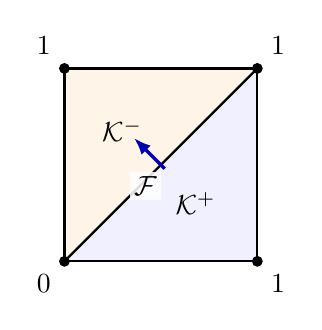
\begin{tikzpicture}[scale=2.45]
  \fill[blue!6] (0,0)--(1,0)--(1,1)--cycle;
  \fill[orange!9] (0,0)--(1,1)--(0,1)--cycle;
  \draw[thick] (0,0) rectangle (1,1);
  \draw[thick] (0,0)--(1,1);
  \foreach \x/\y in {0/0,1/0,1/1,0/1}{\fill (\x,\y) circle (0.8pt);}
  \node[below left=2pt] at (0,0) {$0$};
  \node[below right=2pt] at (1,0) {$1$};
  \node[above right=2pt] at (1,1) {$1$};
  \node[above left=2pt] at (0,1) {$1$};
  \node at (0.68,0.30) {$\mathcal K^+$};
  \node at (0.30,0.68) {$\mathcal K^-$};
  \draw[-{Latex[length=2.2mm]},very thick,blue!70!black]
    (0.52,0.48)--(0.36,0.64);
  \node[fill=white,fill opacity=0.86,text opacity=1,inner sep=1.5pt]
    at (0.42,0.39) {$\mathcal F$};
\end{tikzpicture}

\vspace{0.1cm}
$\displaystyle \bn_{\mathcal F}=\frac{(-1,1)}{\sqrt2}$
\end{column}
\begin{column}{0.55\textwidth}
On each triangle, the $P_1$ function is determined by its three nodal values:
\[
  u_h^+(x,y)=x,
  \qquad
  u_h^-(x,y)=y.
\]
Therefore,
\[
  \grad u_h^+=(1,0),
  \qquad
  \grad u_h^-=(0,1).
\]
Because $f=0$ and these gradients are constant,
\[
  r_\pm=\divg(\grad u_h^\pm)=0.
\]
The estimator would be zero if it contained only element residuals.
\end{column}
\end{columns}
\end{frame}

\begin{frame}{Compute the facet term and the local indicators}
Using the normal shown on the previous slide,
\[
\begin{aligned}
  j_{\mathcal F}
  &=-\bigl(\grad u_h^+-\grad u_h^-\bigr)\cdot\bn_{\mathcal F} \\
  &=-\bigl((1,0)-(0,1)\bigr)\cdot
      \frac{(-1,1)}{\sqrt2}
   =\sqrt2.
\end{aligned}
\]
The diagonal has length $h_{\mathcal F}=\sqrt2$, so
\[
  \norm[L^2(\mathcal F)]{j_{\mathcal F}}^2
  =\int_{\mathcal F}2\,\dd s=2\sqrt2,
  \qquad
  \eta^2=h_{\mathcal F}
  \norm[L^2(\mathcal F)]{j_{\mathcal F}}^2=4.
\]
The shared-facet contribution is divided equally between its two neighboring
elements:
\[
  \eta_+^2=\eta_-^2=2,
  \qquad
  \eta^2=\eta_+^2+\eta_-^2.
\]

The computed function is continuous, but its gradient is not. The facet
residual detects this defect; an element-residual-only estimator would miss it.
\end{frame}

\begin{frame}{Cauchy--Schwarz combines all weighted terms}
Substituting $w=e-\Qh e$ in the residual representation and using the two
local bounds gives a sum of products. Cauchy--Schwarz for that finite sum
gives
\[
\begin{aligned}
  \norm[a]{e}^2
\leq C_Q\eta
\Bigg(&\sum_e\seminorm[H^1(\omega_e)]{e}^2\\
&+\sum_{\mathcal F\in\Fh^\ast}
\seminorm[H^1(\omega_{\mathcal F})]{e}^2\Bigg)^{1/2}.
\end{aligned}
\]
The first factor is the computable estimator $\eta$. The second factor still
contains the error, but only through its $H^1$ seminorm over overlapping
patches.
\end{frame}

\begin{frame}{Finite patch overlap gives a global error norm}
On a shape-regular mesh, an element belongs to at most a fixed number
$N_{\mathrm{ov}}$ of the patches $\omega_e$ and $\omega_{\mathcal F}$.
Consequently,
\[
  \sum_e\seminorm[H^1(\omega_e)]{e}^2
  +\sum_{\mathcal F\in\Fh^\ast}
   \seminorm[H^1(\omega_{\mathcal F})]{e}^2
  \leq N_{\mathrm{ov}}\seminorm[H^1(\Om)]{e}^2.
\]
This is a counting statement: each element contribution to
$\seminorm[H^1(\Om)]{e}^2$ appears in no more than $N_{\mathrm{ov}}$ patches.
Thus
\[
  \norm[a]{e}^2
  \leq C_Q\sqrt{N_{\mathrm{ov}}}\,\eta
  \seminorm[H^1(\Om)]{e}.
\]
\end{frame}

\begin{frame}{Reliability of the residual estimator}
The diffusion coefficient satisfies $k(\bm x)\geq k_0>0$. Hence
\[
  \norm[a]{e}^2
  =\int_\Om k|\grad e|^2\,\dd x
  \geq k_0\seminorm[H^1(\Om)]{e}^2,
\]
and therefore
\[
  \seminorm[H^1(\Om)]{e}
  \leq\frac{1}{\sqrt{k_0}}\norm[a]{e}.
\]
Substituting this inequality into the preceding bound and dividing by
$\norm[a]{e}$ gives
\[
  \boxed{\norm[a]{u-u_h}\leq
  C_Q\sqrt{\frac{N_{\mathrm{ov}}}{k_0}}\,\eta.}
\]
Thus $C_{\mathrm{rel}}=C_Q\sqrt{N_{\mathrm{ov}}/k_0}$. The constant is
independent of the mesh size, although it depends on mesh shape regularity and
the coefficient lower bound.
\end{frame}

\begin{frame}{Reliability and efficiency answer different questions}
\textbf{Reliability} is the global upper bound
\[
  \norm[a]{e}\leq C_{\mathrm{rel}}\eta.
\]
It ensures that a small estimator implies a small energy error.

\textbf{Local efficiency} is a lower-bound statement of the form
\[
  \eta_e\leq C_{\mathrm{eff}}
  \left(\norm[a,\omega_e]{e}+\operatorname{osc}_e\right).
\]
It ensures that a large local indicator is associated with error near
$\mathcal K_e$, apart from the unresolved variation in the prescribed data.
The quantity $\operatorname{osc}_e$, called \textbf{data oscillation},
measures the part of $f$, $q$, or $k$ that is not represented by the local
polynomial data approximation used to evaluate the residual.

Today we proved reliability. Local efficiency requires a separate
lower-bound argument and is not proved in this lecture.
\end{frame}

\begin{frame}{Effectivity measures the scale of an estimator}
When the exact error is available, define the \textbf{effectivity index}
\[
  I_{\mathrm{eff}}
  =\frac{\eta}{\norm[a]{u-u_h}}.
\]
An effectivity index near one means that $\eta$ estimates the magnitude of the
energy error accurately. A nearly constant value different from one means
that the estimator tracks the error but consistently overestimates or
underestimates it.

Effectivity is normally evaluated only in verification problems, because the
exact error is unknown in the applications for which an estimator is needed.

\vspace{0.2cm}
These terms should not be interchanged:
\[
\begin{array}{c|c}
\text{reliability} & \text{the estimator bounds the error from above}\\
\text{efficiency} & \text{the indicator is not unnecessarily large}\\
\text{effectivity} & \text{the observed ratio of estimator to exact error}
\end{array}
\]
\end{frame}

\begin{frame}{Summary and next step}
\begin{itemize}
  \item $R(u_h;v)=a(u-u_h,v)$ connects the computable residual functional to
  the unknown error.
  \item Elementwise integration by parts separates balance defects inside
  elements from flux defects on interior and Neumann facets.
  \item Galerkin orthogonality allows $v$ to be replaced by
  $v-\Qh v$; local approximation then supplies the powers of the local mesh
  size.
  \item The indicators $\eta_e$ identify where the residual is concentrated,
  while reliability bounds the global energy error by $\eta$.
\end{itemize}

\vspace{0.2cm}
\textbf{Exit question.} For $P_1$ elements with elementwise-constant $k$ and
$f=0$, can $\eta$ still be nonzero? Identify the residual term that remains.

\vspace{0.2cm}
\textbf{Next lecture.} Use the local indicators to mark elements, refine the
mesh conformingly, and repeat the solve--estimate--mark--refine loop.
\end{frame}

\end{document}
